\documentclass[conference]{IEEEtran}
\IEEEoverridecommandlockouts
% The preceding line is only needed to identify funding in the first footnote. If that is unneeded, please comment it out.
\usepackage{cite}
\usepackage{amsmath,amssymb,amsfonts}
\usepackage{algorithmic}
\usepackage{graphicx}
\usepackage{textcomp}
\usepackage{xcolor}
\usepackage{subcaption}
\def\BibTeX{{\rm B\kern-.05em{\sc i\kern-.025em b}\kern-.08em
    T\kern-.1667em\lower.7ex\hbox{E}\kern-.125emX}}
\begin{document}

\title{Concurrent IC Global Routing with Multi-Agent Deep Reinforcement Learning}

\author{\IEEEauthorblockN{Shidi Xi}
\IEEEauthorblockA{\textit{Department of Electrical and Computer Engineering} \\
\textit{The University of British Columbia}\\
Vancouver V6T 1Z4, Canada \\
xsd99@ece.ubc.ca}
}

\maketitle

\begin{abstract}
    Global routing is a pivotal stage in integrated circuit (IC) physical design, characterized by its complexity and criticality. Conventional routing methods, which are typically sequential and heuristic-guided, are straightforward to implement but are not immune to the net-ordering problem. This issue arises when nets routed at later stages encounter increased blockages. In this study, a novel approach utilizing multi-agent deep reinforcement learning is introduced to address the IC global routing challenge. The framework models global routing as a pathfinding task on a grid graph, where each net is routed by a distinct agent. These agents, operating cooperatively under a shared super policy, enable concurrent net routing. This collaborative mechanism optimizes the total overflow and wirelength across the entire netlist. Evaluation results demonstrate that the proposed framework outperforms the sequential A* baseline in reducing both overflow and wirelength, marking a significant advancement in global routing solutions.
\end{abstract}

\begin{IEEEkeywords}
    routing, machine learning, multi-agents systems, optimization
\end{IEEEkeywords}

\section{Introduction}
Physical design is a crucial phase in the IC design process, wherein the logical representation of the chip is converted into a physical geometric layout essential for fabrication foundries. This stage is subdivided, with global routing being a key step where pins specified by netlists are connected coarsely using wires and vias. The quality of global routing, often evaluated by total wirelength and edge overflow, impacts vital chip metrics like performance, power, and area \cite{Hu2001}.

Global routing, despite its significance, poses considerable challenges \cite{Liao2020}. The number of nets to be routed can be substantial, and each net may comprise multiple individual pins. Even the simplest version of this problem, involving the routing of a set of 2-pin nets under design constraints, is NP-complete \cite{Kramer1984}. Hence, global routing algorithms aim for a balance between quality and speed. These algorithms also find applications beyond IC design, benefiting areas like network design \cite{Fortz2000} and urban planning \cite{Fragiadakis2015} where optimizing connections and pathways under constraints is crucial.

Traditional global routing often involves decomposing multi-pin nets into 2-pin sub-nets, sequentially routed using maze-routing algorithms like A*. Decomposition typically involves constructing a minimum spanning tree from the pins. Despite the simplicity and efficacy of this approach, the net-ordering issue persists. Later routed nets face increased blockages leading to edge overflow, while early-stage nets lack foresight to conserve resources for subsequent nets. Designers typically resort to rip-up and reroute strategies, where congested pathways are removed and re-routed.

Deep reinforcement learning (DRL), a fusion of reinforcement learning and deep neural networks, has gained prominence in machine learning, showcasing capacities to exceed human performance in various contexts \cite{Mnih2013}. Its application to global routing has yielded promising outcomes, surpassing conventional methods \cite{Liao2020,Xu2023}. Nonetheless, most DRL systems employ a single agent for routing, inheriting the net-ordering problem characteristic of sequential methods.

This work explores the utilization of multi-agent deep reinforcement learning (MADRL) in global routing. In this approach, each net is assigned a dedicated agent for routing, and all agents operate concurrently, guided by a shared super policy. This mitigates the net-ordering issue, as the policy collects data from individual agents, directing them to minimize total overflow and wirelength across the whole netlist. Evaluation demonstrates enhanced performance over the A* baseline.

The subsequent sections provide a detailed exploration. Section 2 outlines the core concepts of global routing and MADRL. Section 3 and 4 delve into problem definition and the intricacies of the MADRL system. Evaluation outcomes and discussions are presented in Section 5. Section 6 outlines the challenge and limitation of this work which paves the road for future works, leading to the conclusion in Section 7.

\section{Preliminaries}
\subsection{Global Routing}
Given a chip placement like Figure \ref{fig:gr}(a), global routing tessellates the chip area into rectangular tiles called G-cells. It can then be represented by a grid graph $G(V, E)$, where each node $v_{i} \in V$ represents one corresponding G-cell, like node A and B in Figure \ref{fig:gr}(b) to cell A and B in (a). And each edge $e_{ij} \in E$, connecting node $v_{i}$ and $v_{j}$, 
represents the routing channel between the two G-cells. Wires connect pins in difference cells using the channels between them. Constrained by design rules, 
each channel can only permit a limit number of wires, called the capacity. Hence, in the grid graph, each edge $e_{ij}$ is assigned a weight $c_{ij}$, representing its capacity. After routing, a case may occur that for some edges, the numbers of wires crossing them exceed their capacities. In this case, these edges have an overflow $O_{ij}$. Suppose an edge has a capacity of 3, and after routing, there are 4 wires crossing it, then there is an overflow of 1. Another important parameter is the wirelength, which is the total number of edges consisting a wire. The scope of global routing is to connect all pins while minimizing the total overflow and wirelength. In this project, the focus is on 2D global routing for simplicity, with all components situated on a single layer. In a real IC physical design process, global routing is three-dimensional, however, the concept of 2D can be easily transferred to 3D.

\begin{figure}[h!]
    \centering
    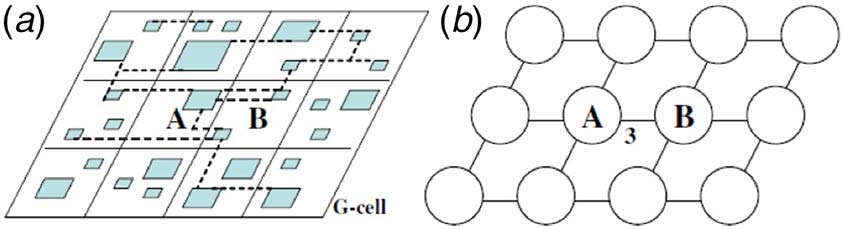
\includegraphics[width = 0.48\textwidth]{figures/gr.jpg}
    \caption{(a) A circuit placement tessellated into G-cells. (b) The abstracted grid graph \cite{Cho2006}.}
    \label{fig:gr}
\end{figure}

\subsection{Multi-agent Deep Reinforcement Learning}
Reinforcement learning (RL) is a sub-field of machine learning. It is essentially a Markov decision process that involves an agent interacting with an environment and making a sequence of decisions. As shown in Figure \ref{fig:rl}, the agent takes an action $a \in A$ to the environment, and receives two signals in return: the state $s \in S$ and the reward $r$. The former provides some information about the environment to the agent, and the latter tells how good was the agent's previous action to some extent. We will shortly see the metric that evaluates the agent's actions more accurately. This cycle of executing an action $a_{t}$, observing state $s_{t}$ and reward $r_{t}$, and choosing a new action $a_{t+1}$ repeats multiple times until the agent observes an terminate state or the process is stopped by the user \cite{SB}.

\begin{figure}[h!]
    \centering
    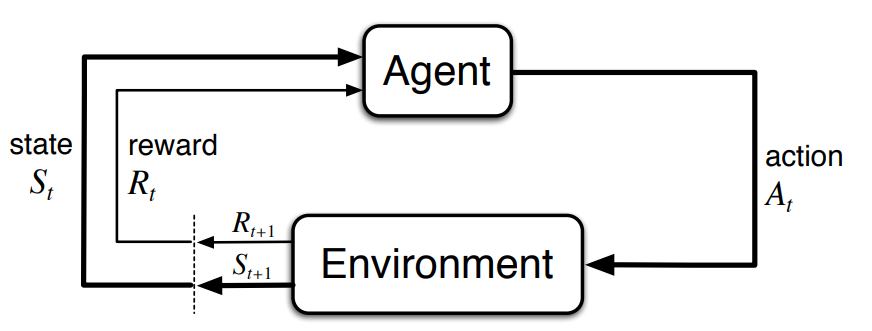
\includegraphics[width = 0.48\textwidth]{figures/rl.png}
    \caption{The agent-environment interaction in a reinforcement learning model \cite{SB}.}
    \label{fig:rl}
\end{figure}

During the process, the agent's objective is to choose a sequence of actions that maximizes the cumulative reward $\sum_{t=0} r_{t}
$ it receives from the environment. One of the methods it can achieve so is to obtain a policy $\pi:S \rightarrow A$, which is a function that maps states to actions (given a state $s_{t}$, the agent takes the corresponding action $a_{t+1}$). Quite often, this mapping function can be very challenging to obtain because the action and the state spaces are very large. A deep neural network can be implemented as a function approximator (the policy network). This combination of deep neural networks and reinforcement learning is referred to as DRL. The policy network takes a state as the input and outputs an action, 
given the environment is deterministic, which is the case for global routing.

The policy network must be trained such that the agent's cumulative reward is maximized. For each action executed, the agent needs feedback on the effectiveness of that action, such that it can adjust the network weights to favour more promising actions as the training proceeds. For this purpose, we define the action-value function $Q_{(s,a)}$, or simply, the Q-value.
\begin{equation} \label{eq:q}
    Q_{(s,a)} = E_{\pi}(r_{t}+\gamma r_{t+1}+\gamma^2 r_{t+2}+...|s_{t} = s, a_{t} = a)
\end{equation}
The Q-value represents the expected cumulative future rewards for taking action $a$ in state $s$ and following policy $\pi$ thereafter. The terms inside the expectation $E_{\pi}$, $r_{t}+\gamma r_{t+1}+\gamma^2 r_{t+2}+...$, represent
the cumulative future rewards from the current time step onwards. Notice that each subsequent future reward is discounted by a factor $\gamma$, which is between 0 and 1. Essentially, the Q-value quantifies how good is it to take an action $a$, given the agent is in state $s$. Not surprisingly, it can be also approximated by a deep neural network, namely, the value network.

The value network assesses the actions selected by the policy network, which then utilizes the feedback for self-improvement such that it will choose actions with higher values in the future. The training procedures are typically:
\begin{itemize}
    \item[(1)] Experience Sampling: The agent interacts with the environment, executing actions, and observing the states and rewards. It collects experience tuples consisting of the current state, executed action, received reward, and the subsequent state.
    \item[(2)] Learning:
    \begin{itemize}
        \item Value Learning: The value network estimates the Q-values of state-action pairs based on the collected experiences, it then provides the values to the policy network. At the same time, the network weights are updated by using methods like stochastic gradient descent. 
        \item Policy Learning: The policy network is updated using methods like stochastic gradient descent that aims to increase the probability of actions with higher Q-values, guided by feedback from the value network.
    \end{itemize}
    
    \item[(3)] Balance between Exploitation and Exploration: The agent exploits the current policy to choose actions that are deemed promising, while also incorporating mechanisms to explore new actions. Exploration ensures the discovery of actions that might be more beneficial but are not yet recognized by the current policy. Strategies like $\epsilon$-greedy can be applicable.
    
    \begin{itemize}
        \item $\epsilon$-greedy algorithm: With a probability of $1-\epsilon$, the agent selects an action according to the current policy. With a probability of $\epsilon$, a random action is chosen to explore new possibilities and escape local optima.
    \end{itemize}
    
    \item[(4)] Iterate: The agent iteratively undergoes the aforementioned steps. The value network's evaluations guide the refinement of the policy network, ensuring a continuous enhancement in the decision-making process to maximize cumulative reward.
\end{itemize}

When there exists multiple agents that interact with an environment simultaneously, it is called multi-agent deep reinforcement learning. Such situation is pervasive in real world's applications. For instance, multiple autonomous vehicles driving on a road, where each one is controlled by an individual RL agent. This kind of implementation is more natural than single agent in some problem contexts. Revisiting the autonomous vehicles example, imagine a future city of ten million self-driving cars. It sounds more feasible for each car to be controlled by one distinct agent than to have a single super agent that collects and computes data from all of the cars simultaneously, in real time. Depending on the context, individual agents can be fully cooperative, fully competitive, or something in between. Fully cooperative MADRL means all agents are altruistic and they take actions that optimize the sum of individual agent's reward (the global reward). These agents may share a single global policy that gathers the actions of individual agents and consider their joint effect on the global reward, as shown in Figure \ref{fig:marl}(a). On the other hand, fully competitive MADRL is when all agents are selfish and they behave in order to maximize their own rewards. Often, they are governed by multiple individual policies that only consider individual actions, as shown in Figure \ref{fig:marl}(b).

\begin{figure}[h!]
    \centering
    \begin{subfigure}[b]{0.48\textwidth}
        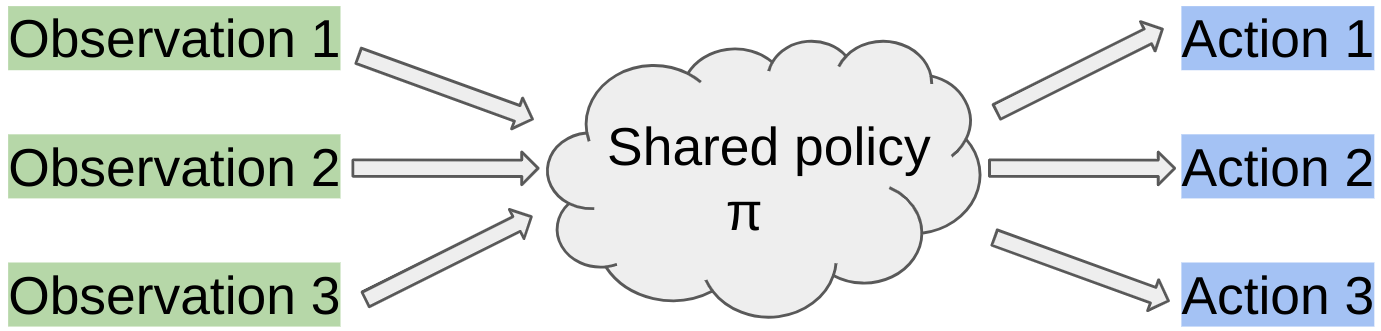
\includegraphics[width=\textwidth]{figures/coop.png}
        \caption{}
    \end{subfigure}
    \hfill % or use \quad
    \begin{subfigure}[b]{0.48\textwidth}
        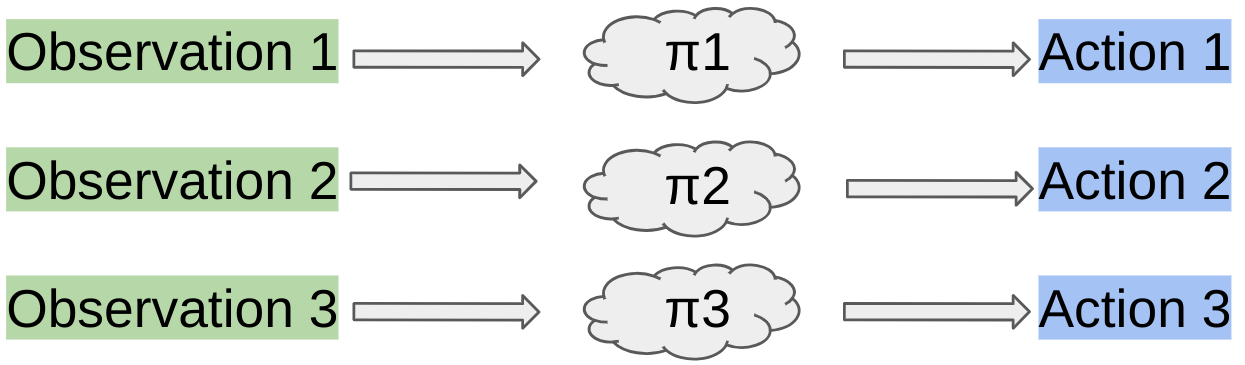
\includegraphics[width=\textwidth]{figures/comp.png}
        \caption{}
    \end{subfigure}
    \caption{Multi-agent reinforcement learning with (a) fully cooperative agents with a shared policy, 
    (b) fully competitive agents with individual policies.}
    \label{fig:marl}
\end{figure}

\section{Global Routing Based on Multi-agent Deep Reinforcement Learning}
In the context of the global routing problem, a netlist, which comprises an arbitrary number of nets with each specifying a set of pins to be connected, is considered. This essentially transforms into a pathfinding challenge on the grid graph. The proposed MADRL framework addresses this challenge, assigning each agent the task of routing a net—initiating from the source nodes and proceeding towards the target nodes. All agents are structured to be fully cooperative, orchestrated by a shared policy. Their united objective targets minimizing two pivotal metrics: the total overflow and the total wirelength encompassing all nets within the netlist.

With a netlist containing $n$ nets, the MADRL router will incorporate $n$ agents. All agents, acting concurrently, are governed by a policy network that processes $n$ states and yields $n$ corresponding actions.

The subsequent sections elaborate on the critical elements of the MADRL router, including state encoding, action space, reward function, and the environmental design. The following discussions will be based on single agent RL for simplicity, however, all agents in the MADRL router are homogeneous, that is, having the same state encoding, action space, etc. Hence, 
the concepts of single agent RL can be easily scaled to multi-agent scenario as it is simply $n$ copies of a single agent. 

\subsection{State Encoding}
A state is a piece of information from the environment represents the current situation of the agent. In the proposed framework, the state is encoded as an 8-dimensional vector. The first two elements $s_{t}[0:1]$ encode the (x,y) 
coordinates of the agent's current position on the grid graph. $s_{t}[2:3]$ represent the coordinates of the agent's target node on the grid graph. 
$s_{t}[4:7]$ depict the capacities of the four edges (up, right, down, left) connected to the agent's current node. This state encoding contains information about the agent's current position, its destination, and the local 
capacity information. 

\subsection{Action Space}
The actions are encoded by an integer ranges from 0 to 3, meaning the agent goes up, right, down, or left from its current position.
\subsection{Reward Function}
The environment imposes a -1 penalty on the agent for each step taken that does not lead to the target, fostering a drive to discover the shortest path. Reaching the target yields a +100 reward, formulated as
\begin{equation} \label{eq:reward}
r_{t+1}(a_{t}, s_{t+1}) =
\begin{cases}
+100 & \text{if \(s_{t+1}[0:1] = s_{t+1}[2:3]\)} \\
-1 & \text{otherwise}
\end{cases}
\end{equation}
This configuration incites the agent to minimize wirelength, equating to the distance traveled to reach the target. Unnecessary deviations culminate in diminished cumulative rewards.

\subsection{Environment Design}
The environment can be viewed as a "black box" that takes input $a_{t}$ and produces output $s_{t+1}$ and $r_{t+1}$. It stores the information about the grid graph, including the grid size, the netlist, the agent's traversed path (the routed wire), and the capacity details. Utilizing this information, the environment calculates the state and associated reward for a given action. Upon receipt of an action from the agent, the environment engages in a series of steps to determine the validity of the action and to compute the subsequent state and reward. The process is outlined as follows:
\begin{itemize}
    \item[(1)] Capacity Check: The environment evaluates whether the action seeks to use an edge with zero capacity. In such instances, the action is deemed invalid. For instance, should the agent attempt a move from node $v_i$ to $v_j$ and the connecting edge $e_{ij}$ has a capacity $c_{ij}$ of zero, the action is prohibited. This design element ensures that the MADRL router is intrinsically hard-coded to prevent overflow.
    \item[(2)] Boundary Check: A verification is conducted to inspect if the agent's new position post-action extends beyond the grid's boundaries. Actions resulting in such an outcome are invalidated.
    \item[(3)] State and Path Update: Provided the action passes the initial checks, the environment calculates the new state $s_{t+1}$. Concurrently, it reduces the capacity of the utilized edge by one and updates the agent’s traversed path accordingly.
    \item[(4)] Reward Calculation: The environment computes the reward $r_{t+1}$ utilizing Equation \ref{eq:reward} and presents the updated state and reward to the agent.
\end{itemize}

\section{A* Baseline}
An A* baseline is developed in parallel with the MADRL framework to serve as a baseline for evaluating the router’s performance. In this setup, nets are routed sequentially, following the order they are parsed into the program. The A* algorithm considers edge capacities; after each net is routed, the capacities of the used edges are reduced accordingly. Edges depleted to zero capacity are treated as obstacles, prompting the algorithm to circumvent them while seeking the shortest path to the destination.

This sequential routing implies that nets addressed later encounter more constraints due to already depleted resources, potentially rendering them unroutable. In such instances, the algorithm relaxes capacity restrictions, allowing the completion of routing at the expense of incurring overflow.

\section{Experimental Results}
The proposed MADRL framework is executed in Python, leveraging the RLlib library for implementation. Proximal policy optimization (PPO) \cite{Schulman2017} is employed for RL training, utilizing the default neural network architectures supplied by RLlib.

Using an open-source problem generator \cite{Liao2020}, 20 problems were created. Each problem is characterized by 35 nets, each with only 2 pins, an 8x8 chip size, and an initial edge capacity of 3. These specific settings facilitate a compact grid and straightforward routing scenarios. Consequently, RL agents can quickly complete the routing, with the entire training process wrapping up in under an hour on a Linux workstation. This workstation is equipped with an Intel Core i5-11300H 8-core CPU, clocked at 3.3 GHz, and 16 GB of RAM.

Given the substantial number of nets and the restricted edge capacity, overflows are evident in some of the A* solutions, while others are free from this issue. The MADRL router's performance is evaluated and compared against the A* baseline across these diverse problem scenarios.

\subsection{Evaluation}
Table \ref{tab:result} summarizes the routing outcomes for the 20 netlists when processed by both the A* baseline and MADRL router. The MADRL router demonstrates the ability to optimize wirelength across both problem types, achieving a 2.6\% average reduction compared to the A* baseline. Notably, the MADRL approach effectively eliminates the overflow issue, successfully routing all problems without this complication.

The visual representation of the routing solutions for problem \#17 is provided in Figure \ref{fig:result}. These heat maps, detailing the utilization of edges, are instrumental in highlighting the comparative efficiency of MADRL over the A* algorithm. The overflow evident in the A* solutions (represented by negative numbers on the heat maps) is conspicuously absent in the MADRL outcomes, attesting to its superior management of overflow and optimization of wirelength.

\begin{table*}[h!]
    \caption{Evaluation results for problems with and without A* overflow.}
    \centering
    \begin{tabular}{|c c c c c|}
        \hline
        \hline
        Problem & A* overflow & A* wirelength & MADRL wirelength & MADRL wirelength \% reduction \\
        \hline
        1 & 0 & 188 & 184 & 2.1\% \\
        2 & 0 & 145 & 149 & -2.8\% \\
        3 & 0 & 161 & 161 & 0.0\% \\
        4 & 0 & 205 & 193 & 5.9\% \\
        5 & 0 & 182 & 180 & 1.1\% \\
        6 & 0 & 151 & 147 & 2.6\% \\
        7 & 0 & 160 & 160 & 0.0\% \\
        8 & 1 & 190 & 182 & 4.2\% \\
        9 & 1 & 198 & 200 & -1.0\% \\
        10 & 1 & 212 & 198 & 6.6\% \\
        11 & 2 & 210 & 208 & 1.0\% \\
        12 & 3 & 208 & 194 & 6.7\% \\
        13 & 3 & 228 & 196 & 14.0\% \\
        14 & 3 & 188 & 200 & -6.4\% \\
        15 & 4 & 174 & 172 & 1.1\% \\
        16 & 6 & 195 & 193 & 1.0\% \\
        17 & 8 & 203 & 195 & 3.9\% \\
        18 & 10 & 208 & 206 & 1.0\% \\
        19 & 13 & 195 & 193 & 1.0\% \\
        20 & 14 & 227 & 207 & 8.8\% \\
        average & - & - & - & 2.6\% \\
        \hline
        \hline
    \end{tabular}
    \label{tab:result}
    \end{table*} 

\begin{figure*}[h!]
    \centering
    \begin{subfigure}[b]{0.31\textwidth}
        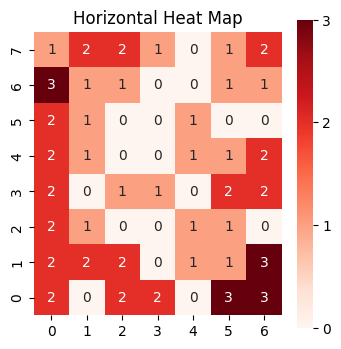
\includegraphics[width=\textwidth]{figures/rl_hhm.png}
        \caption{}
    \end{subfigure}
    \begin{subfigure}[b]{0.35\textwidth}
        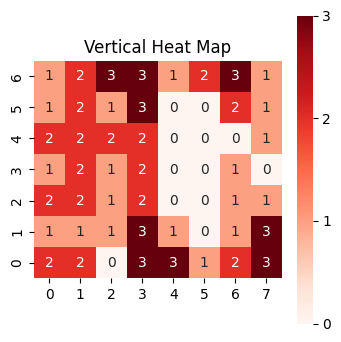
\includegraphics[width=\textwidth]{figures/rl_vhm.png}
        \caption{}
    \end{subfigure}
    \begin{subfigure}[b]{0.31\textwidth}
        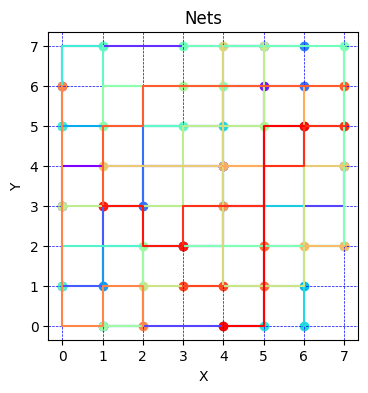
\includegraphics[width=\textwidth]{figures/rl_solution.png}
        \caption{}
    \end{subfigure}
    \begin{subfigure}[b]{0.31\textwidth}
        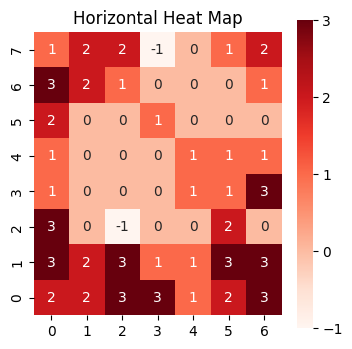
\includegraphics[width=\textwidth]{figures/as_hhm.png}
        \caption{}
    \end{subfigure}
    \begin{subfigure}[b]{0.35\textwidth}
        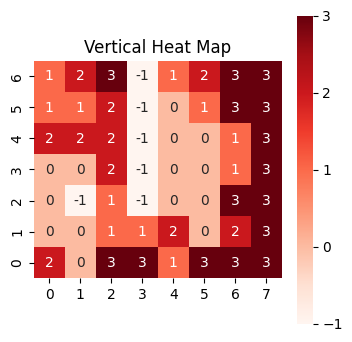
\includegraphics[width=\textwidth]{figures/as_vhm.png}
        \caption{}
    \end{subfigure}
    \begin{subfigure}[b]{0.31\textwidth}
        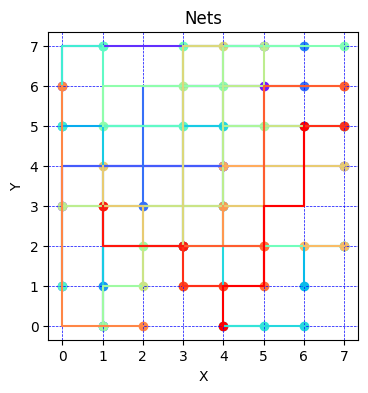
\includegraphics[width=\textwidth]{figures/as_solution.png}
        \caption{}
    \end{subfigure}
    \caption{Visualized routing solutions for problem \#17. (a) MADRL Horizontal heat map. 
    (b) MADRL vertical heat map. (c) MADRL routed nets. (d)-(f) A* solution.}
    \label{fig:result}
\end{figure*}

\subsection{Analysis and Discussion}
The MADRL router's enhanced performance over the A* baseline can be attributed to several key factors.
\begin{itemize}
    \item[(1)] Concurrent Routing of All Nets: In the MADRL approach, nets are not subjected to the hierarchical routing seen in sequential methods like A*. Every net is considered simultaneously, eliminating the issue of later-routed nets encountering increased blockages.
    \item[(2)] Exploration Mechanism: While A* is guided by deterministic heuristics, always opting for the shortest path, RL employs exploration mechanisms, such as the $\epsilon$-greedy algorithm. This approach allows agents to occasionally veer off the optimal path to explore the environment. It fosters the discovery of areas on the grid graph rich in edge capacities, enabling more effective resource utilization. Figure \ref{fig:result}(b) and (e) exemplify this, showcasing underutilized edges in the A* heatmap and optimized edge resource allocation in the RL heatmap.
    \item[(3)] Global Optimization through Cooperative Setting: The fully cooperative setting of MADRL, where all agents are orchestrated by a single shared policy, facilitates global optimization. Every agent is altruistic, potentially sacrificing its own benefit to enhance the overall system's performance. It is not uncommon for an agent to take a longer route to leave room for other nets, reducing individual efficiency but optimizing total wirelength and overflow for the entire netlist. The decision-making process is influenced by the expected cumulative future reward or Q-values (Equation \ref{eq:q}), balancing immediate and long-term rewards and leading to globally optimized outcomes.
\end{itemize}

\section{Challenges and Future Directions}

A prominent challenge of the MADRL framework is the lack of policy generalization to unseen yet similar problems. Currently, a distinct policy must be trained from scratch for each new netlist, which is not time-efficient.

This limitation arises primarily due to the partial observability of the environment induced by the state encoding, which encapsulates only local capacity information. It’s akin to navigating in dense fog, where visibility is limited to the immediate surroundings. Incorporating graph neural networks (GNNs) as state encoders, as suggested by \cite{Mirhoseini2021}, could enhance policy generalization.

Additionally, the use of multilayer perceptrons for architecting policy and value networks may not be optimal for problems modeled as graphs. Existing literature \cite{Almasan2022,Wang2018} highlights the effectiveness of employing GNNs directly within policy and/or value networks for deep RL, promising enhancements in policy generalization.


\section{Conclusion}
This work introduces a multi-agent deep reinforcement learning methodology for IC global routing, conceptualized as a pathfinding problem on a grid graph. The MADRL router, evaluated using 20 benchmarks derived from an open-source generator, demonstrates notable performance. By concurrently routing all nets with fully cooperative agents, it markedly surpasses the sequential A* baseline in terms of preventing edge overflow. Additionally, it optimizes wirelength by an average of 2.6\%.

A prevailing challenge is the lack of generalization of the trained RL policies to new, unseen problems. This limitation is attributed to the current state encoding design and the architectures of the policy and value networks. Addressing this challenge, enhancing the adaptability and efficiency of the MADRL approach, is earmarked as the primary focus for future research endeavors.


\bibliographystyle{IEEEtran}
\bibliography{bibliography}

\end{document}
